\documentclass[aspectratio=169,10pt]{beamer}

\usetheme{Madrid}
\usecolortheme{default}
\setbeamertemplate{navigation symbols}{}
\setbeamertemplate{footline}[frame number]

\usepackage{amsmath,amssymb,amsthm,booktabs,mathtools}
\usepackage{hyperref}
\usepackage{tikz}
\usetikzlibrary{arrows.meta,positioning,decorations.pathreplacing}

% Macros
\newcommand{\F}{\mathbb{F}}
\newcommand{\B}{\{0,1\}}
\newcommand{\eq}{\mathrm{eq}}
\newcommand{\wt}[1]{\widetilde{#1}}
\newcommand{\Perm}{\mathrm{PERM}}
\newcommand{\bigO}{\mathcal{O}}
\newcommand{\polylog}{\mathrm{polylog}}
\DeclareMathOperator{\MLE}{MLE}

\title[Linear-Time Permutation Check]{Linear-Time Permutation Check}
\subtitle{B\"unz, Chen \& DeStefano (2025)}
\author{[name]}
\institute{Shanghai Jiao Tong University}
\date{\today}

\begin{document}

% ============================================================
% TITLE
% ============================================================
\begin{frame}
  \titlepage
\end{frame}

% ============================================================
% ROADMAP
% ============================================================
\begin{frame}{Roadmap}
\begin{enumerate}
  \item \textbf{Motivation}: Why do we need better permutation checks?
  \item \textbf{Key insight}: The arithmetization spectrum of $\wt{1}_\sigma$
  \item \textbf{BiPerm}: Linear-time via 2-way split (sparse PCS only)
  \item \textbf{MulPerm}: Near-linear-time via $\ell$-way split (any PCS)
  \item \textbf{Extensions}: Prover-provided permutation \& lookups
  \item \textbf{Applications}: Improving HyperPlonk \& Spartan
\end{enumerate}
\end{frame}

% ============================================================
% PART 1: WHAT & WHY
% ============================================================

\begin{frame}{Permutation Check: A Core SNARK Primitive}
Given $f, g : \B^\mu \to \F$ and a permutation $\sigma : \B^\mu \to \B^\mu$, prove
\[
  f(x) = g(\sigma(x)) \quad \forall\, x \in \B^\mu, \qquad n = 2^\mu.
\]

\vspace{0.8em}
\textbf{Where does this appear?}
\begin{itemize}
  \item \textbf{Circuit wiring}: Plonk/HyperPlonk copy constraints
  \item \textbf{Memory checking}: RAM-to-sorted-access consistency
  \item \textbf{Lookup arguments}: Table lookups as a special case
\end{itemize}

\vspace{0.8em}
$\Rightarrow$ Prover cost of permutation check \textbf{dominates} overall SNARK prover time.
\end{frame}

\begin{frame}{Prior Art I: Grand Product (Plonk)}
\textbf{Core idea} [GWC19]: $f(x) = g(\sigma(x))$ iff for random $\beta, \gamma \leftarrow \F$,
\[
  \prod_{x \in \B^\mu} \bigl(f(x) + \beta \cdot x + \gamma\bigr) = \prod_{x \in \B^\mu} \bigl(g(x) + \beta \cdot \sigma(x) + \gamma\bigr)
\]
Prover builds an \textbf{accumulator} $z : \B^\mu \to \F$ with $z(0) = 1$ and
\[
  z(\text{next}(x)) = z(x) \cdot \frac{f(x) + \beta \cdot x + \gamma}{g(x) + \beta \cdot \sigma(x) + \gamma}, \qquad z(\text{last}) \stackrel{!}{=} 1.
\]

\vspace{0.3em}
\textbf{Drawbacks:}
\begin{itemize}
  \item \textbf{Extra commitment:} Must commit to $z$ --- a size-$n$ vector of \emph{random field elements}. Each $z(x)$ is a product of random ratios $\Rightarrow$ not structured (not in $\{0,1\}$, no sparsity). MSM cost is full $\bigO(n)$ scalar mults with no shortcuts.
  \item \textbf{Soundness $n/|\F|$:} A non-permutation can still satisfy the product check with probability $\le n/|\F|$ (from Schwartz--Zippel on a degree-$n$ univariate). For $n = 2^{32}$, $|\F| = 2^{64}$, this is only $2^{-32}$.
  \item Runtime commitment to $z$ is often the \textbf{bottleneck} of the entire SNARK.
\end{itemize}
\end{frame}

\begin{frame}{Prior Art II: GKR-Style \& HyperPlonk}
\textbf{GKR-style} [Spartan/SPARK]: View the grand product as a depth-$\log n$ circuit, use GKR [GKR08] to verify it.
\begin{itemize}
  \item \textcolor{green!60!black}{Prover $\bigO(n)$} field ops; \textcolor{green!60!black}{no extra commitment} (removes the accumulator)
  \item \textbf{Drawback 1:} $\bigO(\log^2 n)$ rounds, proof size, and verifier time
  \item \textbf{Drawback 2:} Still soundness $n / |\F|$ (inherited from the product check)
  \item \textbf{Drawback 3:} Super-constant round GKR has Fiat--Shamir security concerns [KRS25]; significantly increases prover latency and implementation complexity
\end{itemize}

\vspace{0.4em}
\textbf{HyperPlonk} [CBBZ23]: Sumcheck-based with degree-$\mu$ arithmetization $\wt{1}_\sigma(X,Y) = \prod_{i=1}^{\mu} \eq(\wt{\sigma}_i(X), Y_i)$.
\begin{itemize}
  \item \textcolor{green!60!black}{Better soundness:} $\bigO(\log^2 n / |\F|)$ via Schwartz--Zippel on the sumcheck
  \item \textcolor{red}{Prover $\bigO(n \log^2 n)$:} Degree $\mu$ in $X$ $\Rightarrow$ computing each $\eq$ product costs $\bigO(\mu^2)$ per point
  \item \textcolor{red}{Commits $\mu$ bit-oracles} $\wt{\sigma}_1, \ldots, \wt{\sigma}_\mu$ (each size $n$) during preprocessing
\end{itemize}
\end{frame}

\begin{frame}{This Paper's Contributions}
\begin{center}
\begin{tabular}{lccc}
\toprule
Protocol & Prover & Soundness & PCS requirement \\
\midrule
\textbf{BiPerm} & $\bigO(n)$ & $\bigO(\log n / |\F|)$ & sparse PCS \\
\textbf{MulPerm} & $n \cdot \widetilde{\bigO}(\sqrt{\log n})$ & $\polylog(n) / |\F|$ & any PCS \\
\bottomrule
\end{tabular}
\end{center}

\vspace{0.6em}
\textbf{Key improvements:}
\begin{itemize}
  \item Soundness: $2^{-96} \to 2^{-120}$ for $n = 2^{32}$, $|\F| = 2^{128}$
  \item No commitment beyond the witness (no accumulator/GKR)
  \item $\bigO(\log n)$ verifier and proof size for both
  \item Generalizes to \textbf{lookups} and \textbf{prover-provided} permutations
\end{itemize}
\end{frame}

% ============================================================
% PART 2: KEY INSIGHT
% ============================================================

\begin{frame}{Notation Refresher}
\textbf{Equality polynomial:}
$\eq(a, b) = ab + (1-a)(1-b)$ for $a,b \in \F$.\\
For vectors: $\eq(\mathbf{a}, \mathbf{b}) = \prod_{i=1}^{\mu} \eq(a_i, b_i)$.
Satisfies $\eq(\mathbf{a}, \mathbf{b}) = 1$ iff $\mathbf{a} = \mathbf{b}$ over $\B^\mu$.

\vspace{0.6em}
\textbf{Multilinear extension (MLE):}
For $f : \B^\mu \to \F$, its unique MLE is
$\wt{f}(X) = \sum_{x \in \B^\mu} f(x) \cdot \eq(x, X)$.

\vspace{0.6em}
\textbf{Sumcheck protocol} \textup{[LFKN'90]}:
Proves $\sum_{x \in \B^\mu} f(x) = v$ for degree-$d$ polynomial $f$.\\
Soundness $d\mu / |\F|$; prover sends $\mu$ univariate messages of degree $\le d$.

\vspace{0.6em}
\textbf{Permutation as multilinear map:}
$\sigma : \B^\mu \to \B^\mu$ encoded as $\wt{\sigma}(X) = (\wt{\sigma}_1(X), \ldots, \wt{\sigma}_\mu(X))$, each $\wt{\sigma}_i$ is an MLE with $\wt{\sigma}_i(x) \in \{0,1\}$ over $\B^\mu$.
\end{frame}

\begin{frame}{Reduction to Sumcheck (Lemma 4)}
\textbf{Indicator function:} $1_\sigma(x,y) = \begin{cases} 1 & \text{if } \sigma(x) = y \\ 0 & \text{otherwise} \end{cases}$

\vspace{0.6em}
\textbf{Key reduction:} For random $\alpha \leftarrow \F^\mu$, proving $f(x) = g(\sigma(x))$ for all $x$ reduces to
\[
  \boxed{\sum_{x \in \B^\mu} f(x) \cdot \wt{1}_\sigma(x, \alpha) = g(\alpha)}
\]
via Schwartz--Zippel on $\alpha$.

\vspace{0.8em}
$\Rightarrow$ \textbf{The entire protocol design reduces to choosing the arithmetization of $\wt{1}_\sigma(X, Y)$.}

\vspace{0.4em}
Different arithmetizations $\Rightarrow$ different degrees in $X$ $\Rightarrow$ different prover costs.
\end{frame}

\begin{frame}{The Arithmetization Spectrum}
Two ways to write the indicator $1_\sigma(X,Y)$ as a polynomial:

\vspace{0.2em}
\textbf{Full MLE} ($2\mu$ variables, degree 1 in each $X_i$):
$\wt{1}_\sigma(X,Y) = \sum_{x \in \B^\mu} \eq(x \| \sigma(x),\, X \| Y)$.
Oracle is $n^2$-ambient but only $n$-sparse. After fixing $Y = \alpha$, the slice $T_\alpha(X) = \eq(\sigma(X), \alpha)$ is multilinear $\Rightarrow$ sumcheck with $f \cdot T_\alpha$ has \textbf{degree 2}.

\vspace{0.2em}
\textbf{Factored} (group $\mu$ bit-wise relations into $\ell$ groups, degree $\ell$ in each $X_i$):
$\wt{1}_\sigma(X,Y) = \prod_{j=1}^{\ell} \wt{1}_j(X, Y^{(j)})$. Sumcheck degree $\ell + 1$.

\begin{center}
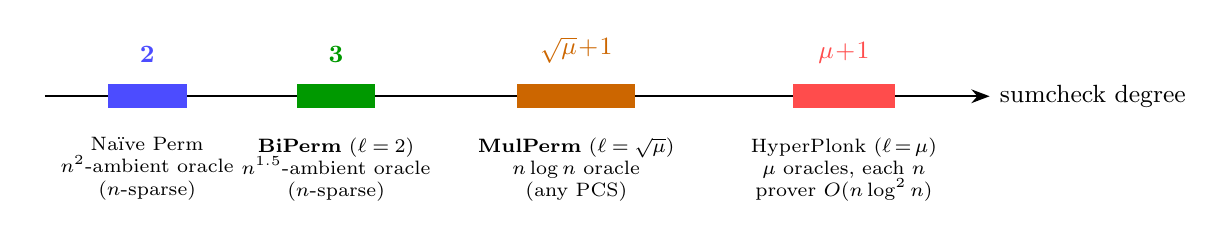
\begin{tikzpicture}[>=Stealth, font=\small]
  \draw[->, thick] (0,0) -- (12,0) node[right] {sumcheck degree};
  % Naive
  \fill[blue!70] (0.8,-0.15) rectangle (1.8,0.15);
  \node[above, blue!70] at (1.3,0.3) {\textbf{2}};
  \node[below, font=\scriptsize, text width=2.8cm, align=center] at (1.3,-0.4) {Na\"ive Perm \\ $n^2$-ambient oracle \\ ($n$-sparse)};
  % BiPerm
  \fill[green!60!black] (3.2,-0.15) rectangle (4.2,0.15);
  \node[above, green!60!black] at (3.7,0.3) {\textbf{3}};
  \node[below, font=\scriptsize, text width=2.5cm, align=center] at (3.7,-0.4) {\textbf{BiPerm} ($\ell\!=\!2$) \\ $n^{1.5}$-ambient oracle \\ ($n$-sparse)};
  % MulPerm
  \fill[orange!80!black] (6,-0.15) rectangle (7.5,0.15);
  \node[above, orange!80!black] at (6.75,0.3) {\textbf{$\sqrt{\mu}\!+\!1$}};
  \node[below, font=\scriptsize, text width=3cm, align=center] at (6.75,-0.4) {\textbf{MulPerm} ($\ell\!=\!\sqrt{\mu}$) \\ $n\log n$ oracle \\ (any PCS)};
  % HyperPlonk
  \fill[red!70] (9.5,-0.15) rectangle (10.8,0.15);
  \node[above, red!70] at (10.15,0.3) {\textbf{$\mu\!+\!1$}};
  \node[below, font=\scriptsize, text width=2.5cm, align=center] at (10.15,-0.4) {HyperPlonk ($\ell\!=\!\mu$) \\ $\mu$ oracles, each $n$ \\ prover $O(n\log^2 n)$};
\end{tikzpicture}
\end{center}

Na\"ive Perm introduces a polynomial with $2\mu$ variables (ambient size $n^2$). The paper argues this leads to ``over linear opening cost during compilation, even with the best known PCS.''
\end{frame}

% ============================================================
% PART 3: BIPERM
% ============================================================

\begin{frame}{BiPerm: The Two-Way Split}
Split $Y = (Y_L, Y_R)$ with $|Y_L| = |Y_R| = \mu/2$. Define
\[
  R_{\sigma_L} = \bigcap_{i \le \mu/2} R_{\sigma_i}, \qquad R_{\sigma_R} = \bigcap_{i > \mu/2} R_{\sigma_i}.
\]

Arithmetize as product of two sub-indicators:
\[
  \wt{1}_\sigma(X, Y) = \wt{1}_{\sigma_L}(X, Y_L) \cdot \wt{1}_{\sigma_R}(X, Y_R)
\]

Substituting into Lemma 4:
\[
  \boxed{\sum_{x \in \B^\mu} f(x) \cdot \wt{1}_{\sigma_L}(x, \alpha_L) \cdot \wt{1}_{\sigma_R}(x, \alpha_R) = g(\alpha)}
\]

This is a \textbf{single sumcheck} with degree 3 in each variable of $x$.
\end{frame}

\begin{frame}{BiPerm: Why the Prover Is $\bigO(n)$}
For $X \in \B^\mu$:
\[
  \wt{1}_{\sigma_L}(X, Y_L) = \sum_{x \in \B^\mu} \eq(x, X) \cdot \eq(\sigma_L(x), Y_L) = \eq(\sigma_L(X), Y_L)
\]

\textbf{Building the evaluation table of $\wt{1}_{\sigma_L}(\cdot, \alpha_L)$ over $\B^\mu$:}
\begin{enumerate}
  \item Precompute $\eq(y_L, \alpha_L)$ for all $y_L \in \B^{\mu/2}$ \hfill $\bigO(2^{\mu/2}) = \bigO(\sqrt{n})$
  \item For each $x \in \B^\mu$: look up $\eq(\sigma_L(x), \alpha_L)$ from the table \hfill $\bigO(n)$
\end{enumerate}
Same for $\wt{1}_{\sigma_R}(\cdot, \alpha_R)$.

\vspace{0.6em}
The sumcheck itself is constant-degree ($\le 3$), so the standard linear-time sumcheck algorithm applies.

\vspace{0.6em}
$\Rightarrow$ \textbf{Total prover: $\bigO(n)$ field operations.}
\end{frame}

\begin{frame}{BiPerm: The PCS Constraint}
The sub-indicators live in $1.5\mu$ variables:
\[
  \wt{1}_{\sigma_L}, \wt{1}_{\sigma_R} : \F^{1.5\mu} \to \F, \qquad \text{table size } 2^{1.5\mu} = n^{1.5}.
\]

But each has only $n$ non-zero entries (= $n$-\textbf{sparse}).

\vspace{0.6em}
\begin{center}
\begin{tabular}{lcc}
\toprule
PCS family & Cost driver & BiPerm compatibility \\
\midrule
Sparse-friendly (Dory, KZH) & sparsity $n$ & \textcolor{green!60!black}{\textbf{good fit}} \\
Dense (KZG, FRI-based) & full table $n^{1.5}$ & \textcolor{red}{\textbf{too costly}} \\
\bottomrule
\end{tabular}
\end{center}

\vspace{0.6em}
\textbf{Theorem 4 (BiPerm).}
\begin{itemize}
  \item Prover: $\bigO(n)$ field ops \quad Verifier: $\bigO(\log n)$ \quad Soundness: $\bigO(\log n / |\F|)$
  \item Index oracles: two $n^{1.5}$-sized sparse polynomials
  \item \textbf{Limitation:} requires sparse PCS for linear prover cost
\end{itemize}
\end{frame}

\begin{frame}{Remark: Does Splitting Actually Help? (``OnePerm'')}
BiPerm's linear prover relies on a simple trick: precompute $\eq(y_L, \alpha_L)$ over $\B^{\mu/2}$, then look up each $\wt{1}_{\sigma_L}(x, \alpha_L) = \eq(\sigma_L(x), \alpha_L)$.

\vspace{0.4em}
\textbf{But the same trick works without splitting.} Define ``OnePerm'':
\begin{enumerate}
  \item Preprocess the full indicator $\wt{1}_\sigma(X,Y) = \sum_{x \in \B^\mu} \eq(x \| \sigma(x), X \| Y)$
  \item After receiving $\alpha$, compute the slice $T_\alpha(x) = \eq(\sigma(x), \alpha)$ for all $x \in \B^\mu$:
    \begin{itemize}
      \item Precompute $\eq(y, \alpha)$ for all $y \in \B^\mu$ \hfill $\bigO(n)$
      \item For each $x$: look up $\eq(\sigma(x), \alpha)$ \hfill $\bigO(n)$
    \end{itemize}
  \item Run a \textbf{degree-2 sumcheck}: $\sum_{x} f(x) \cdot T_\alpha(x) = g(\alpha)$ \hfill $\bigO(n)$
\end{enumerate}

\vspace{0.3em}
\textbf{Comparison with BiPerm:}\\
\begin{center}
\small
\begin{tabular}{lccc}
\toprule
& PIOP prover & Oracle ambient size & Soundness \\
\midrule
``OnePerm'' & $\bigO(n)$ & $n^2$ ($n$-sparse) & $\bigO(\log n / |\F|)$ \\
BiPerm & $\bigO(n)$ & $2 \times n^{1.5}$ ($n$-sparse each) & $\bigO(\log n / |\F|)$ \\
\bottomrule
\end{tabular}
\end{center}

Both need sparse PCS. The only difference is oracle ambient size ($n^2$ vs $n^{1.5}$). With a PCS whose cost depends on \textbf{sparsity} rather than ambient size (e.g.\ Dory, KZH), they are essentially equivalent.
\end{frame}

% ============================================================
% PART 4: MULPERM
% ============================================================

\begin{frame}{MulPerm: Motivation}
\textbf{BiPerm's problem:} The sub-indicators $\wt{1}_{\sigma_L}, \wt{1}_{\sigma_R}$ are committed in preprocessing. Without sparse PCS, commitment cost is $\Omega(n^{1.5})$.

\vspace{0.8em}
\textbf{MulPerm's approach:}
\begin{itemize}
  \item Do \textbf{not} preprocess/commit the sub-indicator functions
  \item Instead, the prover \textbf{computes them at runtime} and \textbf{proves their correctness} via an additional sumcheck
  \item Only preprocessed oracle: $\wt{\sigma}_{[\mu]}$ (size $n \log n$, maps to $\{0,1\}$)
\end{itemize}

\vspace{0.8em}
\textbf{Result:} A ``double-sumcheck'' protocol compatible with \textbf{any} PCS.
\end{frame}

\begin{frame}{MulPerm: $\ell$-Way Factorization}
Partition the $\mu$ output bits into $\ell$ groups of size $\mu/\ell$.

\vspace{0.3em}
Define the \textbf{partial product} polynomial $p : \B^{\mu + \log\ell} \to \F$:
\[
  p(x, \langle j \rangle) := \prod_{i=1}^{\mu/\ell} \eq\!\bigl(\alpha(\langle j' + i \rangle),\; \wt{\sigma}_{[\mu]}(\langle j'+i \rangle, x)\bigr)
\]
where $j' = (j-1)\mu/\ell$ and $\langle j \rangle$ is the $\log\ell$-bit encoding of $j-1$.

\vspace{0.5em}
Let $\wt{p}$ be the MLE of $p$. The permutation check becomes:
\[
  \boxed{\sum_{x \in \B^\mu} f(x) \prod_{j \in [\ell]} \wt{p}(x, \langle j \rangle) = g(\alpha)}
\]

Since $\wt{p}$ is \textbf{not} in the index, the prover must additionally prove $\wt{p}$ is correct $\Rightarrow$ \textbf{second sumcheck}.
\end{frame}

\begin{frame}{Computing $\wt{p}$ Efficiently}
\textbf{Na\"ive cost:} $n\ell \cdot (\mu/\ell) = n\mu$ field multiplications. Too expensive.

\vspace{0.6em}
\textbf{Key observation:} Each $\wt{\sigma}_i(x) \in \{0, 1\}$ over $\B^\mu$, so $\eq(\alpha_i, \wt{\sigma}_i(x)) \in \{\alpha_i,\; 1-\alpha_i\}$ (only 2 possible values).

$\Rightarrow$ For fixed $j$, the product $p(\cdot, \langle j \rangle)$ takes at most $2^{\mu/\ell}$ distinct values across all $x \in \B^\mu$.

\vspace{0.6em}
\textbf{Algorithm (bucketing):}
\begin{enumerate}
  \item Compute all $\ell \cdot 2^{\mu/\ell}$ distinct evaluations \hfill $(\mu/\ell) \cdot \ell \cdot 2^{\mu/\ell}$ mults
  \item For each $(x, j)$: look up the corresponding value \hfill $\bigO(n\ell)$ lookups
\end{enumerate}

\vspace{0.3em}
\textbf{Total Mults:} $\mu \cdot 2^{\mu/\ell} = \mu \cdot n^{1/\ell} = o(n)$ for any $\ell > 1$.
\end{frame}

\begin{frame}{MulPerm: The Double Sumcheck}
\textbf{First sumcheck} (degree $\ell + 1$ in $x$):
\[
  \sum_{x \in \B^\mu} f(x) \prod_{j \in [\ell]} \wt{p}(x, \langle j \rangle) = g(\alpha)
  \quad \xrightarrow{\text{reduces to}} \quad
  \wt{p}(\beta, \langle j \rangle) = P_j \;\;\forall j \in [\ell]
\]
Prover cost: $n \cdot \widetilde{\bigO}(\ell)$ \quad Soundness: $(\ell+1)(\mu + \log\ell) / |\F|$

\vspace{0.8em}
\textbf{Second sumcheck} (degree $\mu/\ell + 1$, proving $\wt{p}$ is correct):
\[
  \sum_{\substack{x \in \B^\mu \\ j \in [\ell]}} \eq(\beta', x \| \langle j \rangle) \underbrace{\prod_{i=1}^{\mu/\ell} \eq\!\bigl(\alpha(\langle j'+i \rangle), \wt{\sigma}_{[\mu]}(\langle j'+i \rangle, x)\bigr)}_{= p(x, \langle j \rangle)} = S_{\wt{p}}
\]
Prover cost: $n \cdot \widetilde{\bigO}(\mu/\ell) + \ell \cdot 2^\ell$
\end{frame}

\begin{frame}{The Bucketing Trick in the Second Sumcheck}
\textbf{Problem:} Degree $\mu/\ell + 1$ is high $\Rightarrow$ na\"ive cost $n \cdot \widetilde{\bigO}(\mu/\ell)$ per round.

\vspace{0.5em}
\textbf{Observation:} In round $k$, each univariate $\wt{\sigma}_{[\mu]}(\langle i \rangle, (\gamma, X, x'))$ has at most $2^{2^k}$ polynomial identities (from $\{0, 1, X, 1-X\}$ possibilities).

$\Rightarrow$ The partial product $p$ has at most $2^{2^k \mu/\ell} \cdot \ell$ distinct polynomial identities.

\vspace{0.5em}
\textbf{Strategy:}
\begin{itemize}
  \item \textbf{Rounds $k < \log\ell$}: Use bucketing --- group terms by polynomial identity, compute eq-sums per bucket. Cost: $\bigO(\mu^2/\ell) \cdot 2^{2^k \mu/\ell}$ mults.
  \item \textbf{Round $k' = \log\ell$}: \# identities exceeds direct computation cost. \textbf{Switch} to standard sumcheck algorithm.
\end{itemize}

\vspace{0.3em}
The switch requires computing collapsed evaluation tables: cost $\ell \cdot 2^\ell$ field ops (Algorithm 11).
\end{frame}

\begin{frame}{The Collapse Algorithm (Algorithm 11)}
\textbf{Goal:} At round $k' = \log\ell$, switch to direct computation.  Need evaluation tables of
$\wt{\sigma}_{[\mu]}\!\bigl(\langle i \rangle, (\gamma, x)\bigr)$ for all $i \in [\mu]$, where $\gamma \in \F^{k'}$ are prior challenges, $x \in \B^{\mu - k'}$.

\vspace{0.4em}
\textbf{Key insight:} $\wt{\sigma}_{[\mu]}(\langle i \rangle, \cdot)$ is $\{0,1\}$-valued on $\B^\mu$.  Each block of $2^{k'}\!=\!\ell$ entries (over the first $k'$ Boolean variables) forms a bit string $s \in \{0,1\}^\ell$.  Only $2^\ell$ possible patterns $\Rightarrow$ precompute all of them.

\vspace{0.4em}
\textbf{Step 1 --- Build lookup table $T$} (size $2^\ell$):\;
For each $s \in \{0,1\}^\ell$, compute $\operatorname{Fold}(s, \gamma)$ --- standard MLE evaluation that iteratively collapses Boolean variables to challenges:
\[
  s'_j \;\leftarrow\; s_j\,(1 - \gamma_i) + s_{|s|/2+j}\,\gamma_i, \qquad i = 1,\ldots,\log\ell
\]
After $\log\ell$ rounds: $\ell \to \ell/2 \to \cdots \to 1$ field element.  Cost per call: $\bigO(\ell)$.

Total table construction: $2^\ell \times \bigO(\ell) = \bigO(\ell \cdot 2^\ell)$ field mults.

\vspace{0.4em}
\textbf{Step 2 --- Lookup:} For each $(i, j)$ with $i \in [\mu]$, $j \in [n/\ell]$: read the $\ell$-bit block from the original evaluation table of $\wt{\sigma}_{[\mu]}(\langle i \rangle, \cdot)$, look up $T[\text{block}]$.  \textbf{Zero} additional field operations.

\vspace{0.3em}
\textbf{Total collapse cost:} $\ell \cdot 2^\ell = \sqrt{\log n} \cdot 2^{\sqrt{\log n}} = o(n)$. \quad Sublinear!
\end{frame}

\begin{frame}{MulPerm: Prover Complexity Analysis}
\textbf{Three components:}
\begin{enumerate}
  \item \textbf{Pre-computation:} evaluate $\wt{p}$ over $\B^{\mu+\log\ell}$ via bucketing (Lemma 5): $\mu \cdot n^{1/\ell} = o(n)$.
  \item \textbf{First sumcheck} (degree $\ell+1$, $\mu$ rounds): $n \cdot \widetilde{\bigO}(\ell)$ field ops.
  \item \textbf{Second sumcheck} (degree $\mu/\ell + 1$, $\mu + \log\ell$ rounds):
  \begin{itemize}
    \item \textit{Bucketing phase} ($k < \log\ell$): round-$k$ cost $\bigO(\mu^2/\ell) \cdot 2^{2^k\mu/\ell}$; geometric $\Rightarrow$ total $\ll n$.
    \item \textit{Collapse} ($k = \log\ell$): $\ell \cdot 2^\ell$ field ops (Algorithm 11).
    \item \textit{Direct phase} ($k > \log\ell$): $n \cdot \bigO(\mu^2/\ell^2) \xrightarrow{\text{FFT}} n \cdot \widetilde{\bigO}(\mu/\ell)$.
  \end{itemize}
\end{enumerate}

\vspace{0.3em}
\textbf{Total:}
\[
  n \cdot \widetilde{\bigO}\!\left(\ell + \frac{\mu}{\ell}\right) + \ell \cdot 2^\ell
  \quad\xrightarrow{\;\ell\,=\,\sqrt{\mu}\;}\quad
  n \cdot \widetilde{\bigO}(\sqrt{\log n})
\]

\textbf{Theorem 5 (MulPerm).}
\begin{itemize}
  \item Prover: $n \cdot \widetilde{\bigO}(\sqrt{\log n})$ \quad Verifier/Proof: $\bigO(\log n)$
  \item Soundness: $\bigO(\mu^{1.5}/|\F|) = \polylog(n)/|\F|$ \quad \textbf{Any PCS}
\end{itemize}
\end{frame}

% ============================================================
% PART 5: EXTENSIONS
% ============================================================

\begin{frame}{Prover-Provided Permutation}
\textbf{Setting:} $\sigma$ is not preprocessed --- e.g.\ memory-checking, where the mapping depends on the witness.

\vspace{0.5em}
\textbf{Prover must additionally show $\sigma$ is a permutation:}

\begin{enumerate}
  \item Provide $\wt{\tau}_{[\mu]}$ (claimed $\sigma^{-1}$)
  \item Prove $\tau(\sigma(y)) = y$ for all $y \in \B^\mu$:
    \[
      \sum_{x \in \B^\mu} x \cdot \wt{1}_\sigma(x, \alpha) = \wt{\tau}(\alpha) \qquad \text{(batched with main permcheck via random $r$)}
    \]
  \item Prove $\sigma$ maps to binaries: $\wt{\sigma}_{[\mu]}(i, x) \in \{0,1\}$ for all $x \in \B^\mu, i \in [\mu]$:
    \[
      \sum_{x \in \B^\mu, i \in [\mu]} \eq((x, \langle i \rangle), s) \cdot \wt{\sigma}_{[\mu]}(i,x)(1 - \wt{\sigma}_{[\mu]}(i,x)) = 0
    \]
\end{enumerate}

\vspace{0.3em}
\textbf{Result (Thm 6):} Triple-sumcheck PIOP, prover $n \cdot \widetilde{\bigO}(\sqrt{\log n})$, soundness $\polylog(n)/|\F|$.
\end{frame}

\begin{frame}{Binary Check: Bucketing Revisited}
\textbf{Goal:} Prove $\wt{\sigma}_{[\mu]}(i, x) \in \{0,1\}$ for all $x \in \B^\mu$, $i \in [\mu]$.

\vspace{0.3em}
Define $h(x, i) := \wt{\sigma}_{[\mu]}(i, x)\bigl(1 - \wt{\sigma}_{[\mu]}(i, x)\bigr)$.  Let $\mu' = \mu + \log\mu$.  Sumcheck:
\[
  \sum_{x' \in \B^{\mu'}} \eq(x', s) \cdot h(x') = 0, \qquad s \leftarrow \F^{\mu'}
\]
Degree 3 in each variable $\Rightarrow$ na\"ive cost $\bigO(n\mu)$ multiplications.

\vspace{0.4em}
\textbf{Trick --- ``Prover buckets in their head'':} Fold the last $b$ variables of $h$ using partial sums with components of $s$:
\[
  h^{(b)}(x', s'') = \sum_{z \in \B^b} h(x' \| z) \cdot \eq(z, s'')
\]
Replace sumcheck target with $\sum_{x' \in \B^{\mu'-b}} \eq(x', s_{[:\mu'-b]}) \cdot h^{(b)}(x', s_{[-b:]}) = 0$.

\vspace{0.4em}
\textbf{Why it helps:} Same as MulPerm --- $\wt{\sigma}_{[\mu]}$ is binary-valued, so in round $k$, $h^{(b)}$ has $\le 2^{2^{b+k}}$ polynomial identities.  Set $b = \log\mu' - k - 2$:
\begin{itemize}
  \item Multiplications: $8 \cdot 2^{2^{\log\mu'-2}} = 8(n\mu)^{1/4}$ per round $\Rightarrow$ $o(n)$ total.
  \item Additions: $2^{\mu' - \log\mu' + 2}$ per round $\Rightarrow$ $\bigO(n \log\log n)$ over $\log\mu'$ rounds.
\end{itemize}
After $\log\mu'$ rounds, switch to direct (Collapse): remaining $o(n)$.

\vspace{0.3em}
\textbf{Lemma 9:} Binary check costs $n \cdot o(\log\log n)$ adds $+$ $o(n)$ mults $\Rightarrow$ \textbf{does not dominate} MulPerm.
\end{frame}

\begin{frame}{Generalization to Lookups}
Replace permutation $\sigma : \B^\mu \to \B^\mu$ with a \textbf{map} $\rho : \B^\mu \to \B^\kappa$ ($T = 2^\kappa$).

Prove: $f(\rho(x)) = g(x)$ for all $x \in \B^\mu$, where $f$ is a $\kappa$-variate table.

\vspace{0.5em}
\textbf{Extra challenge:} $\rho$ is not injective $\Rightarrow$ no inverse, cannot apply Schwartz--Zippel directly on $\alpha$.

\vspace{0.3em}
\textbf{Solution:} Add an outer sum with random $s \in \F^\mu$:
\[
  \underbrace{\sum_{y \in \B^\kappa} f(y) \sum_{x \in \B^\mu} \eq(x,s) \cdot \wt{1}_\rho(x,y)}_{\text{outer sumcheck (exploits sparsity of } 1_\rho\text{)}} = \sum_{x \in \B^\mu} \eq(x,s) \cdot g(x)
\]

After outer sumcheck reduces to a point, apply \textbf{MulPerm} on the inner sum.

\vspace{0.3em}
\textbf{Theorem 7 (MulLookup):} Prover $n \cdot \widetilde{\bigO}(\sqrt{\log T})$ if $T \le n$; soundness $\polylog(n+T)/|\F|$.
\end{frame}

% ============================================================
% PART 6: APPLICATIONS & WRAP-UP
% ============================================================

\begin{frame}{Application: Improving HyperPlonk \& Spartan}
\textbf{HyperPlonk} (copy constraints in Plonk-like systems):
\begin{center}
\begin{tabular}{lccc}
\toprule
Variant & Extra commitments & Prover field ops & PCS \\
\midrule
Original HyperPlonk & $\mu$ bit-oracles & $\bigO(n \log^2 n)$ & any \\
+ BiPerm & 2 sparse oracles & $\bigO(n)$ & sparse \\
+ MulPerm & 1 oracle ($n\log n$) & $n \cdot \widetilde{\bigO}(\sqrt{\log n})$ & any \\
\bottomrule
\end{tabular}
\end{center}

\vspace{0.6em}
\textbf{Spartan / SPARK} (R1CS with sparse matrices):
\begin{itemize}
  \item Sparse matrix $\wt{M}(x,y) = \sum_j \wt{\mathrm{val}}(j) \cdot \wt{1}_{\mathrm{row}}(j,x) \cdot \wt{1}_{\mathrm{col}}(j,y)$
  \item $(\mathrm{row}, \mathrm{col})$ is a preprocessed lookup/permutation object
  \item $\Rightarrow$ Replace memory-checking + GKR by MulPerm-style lookup
  \item Result: avoid GKR entirely, better verifier cost ($\log n$ vs $\log^2 n$)
\end{itemize}
\end{frame}

\begin{frame}{Summary Comparison}
\begin{center}
\small
\begin{tabular}{lcccc}
\toprule
Protocol & Prover & Verifier & Soundness & PCS \\
\midrule
Grand product & $\bigO(n)$+comm & $\bigO(\log n)$ & $n/|\F|$ & any \\
GKR-style & $\bigO(n)$ & $\bigO(\log^2 n)$ & $n/|\F|$ & any \\
HyperPlonk & $\bigO(n\log^2 n)$ & $\bigO(\log n)$ & $\bigO(\log^2 n/|\F|)$ & any \\
\midrule
\textbf{BiPerm} & $\bigO(n)$ & $\bigO(\log n)$ & $\bigO(\log n/|\F|)$ & sparse \\
\textbf{MulPerm} & $n\widetilde{\bigO}(\sqrt{\log n})$ & $\bigO(\log n)$ & $\polylog(n)/|\F|$ & any \\
\bottomrule
\end{tabular}
\end{center}

\vspace{0.6em}
\begin{itemize}
  \item \textbf{BiPerm}: asymptotically optimal prover, but restricted to sparse PCS
  \item \textbf{MulPerm}: universal construction, near-linear, works with any PCS
  \item Both generalize to lookups and prover-provided permutations
\end{itemize}
\end{frame}

\begin{frame}{Open Problems \& Discussion}
\textbf{Open questions from the paper:}
\begin{enumerate}
  \item \textbf{Fully linear} permutation/lookup argument with no PCS dependency?
  \item Reduce soundness error further to \textbf{constant$/|\F|$}?
\end{enumerate}

\vspace{0.8em}
\textbf{Discussion points:}
\begin{itemize}
  \item Is the bucket$\to$direct-computation switch at $k' = \log\ell$ optimal in practice?
  \item For concrete backends (IPA/FRI), where is the HyperPlonk $\leftrightarrow$ MulPerm crossover?
  \item Can the ``small image space $\Rightarrow$ bucketing'' idea be reused in other contexts (e.g.\ GKR layers, memory-checking)?
  \item If sparse PCS is available, does BiPerm dominate once preprocessing is amortized?
\end{itemize}

\vspace{0.8em}
\centering
\small Reference: B\"unz, Chen \& DeStefano, \emph{Linear-Time Permutation Check}, 2025.
\end{frame}

\end{document}
